\documentclass[12pt,a4paper]{report}
\usepackage{amsmath}
\usepackage{amsfonts}
\usepackage{amssymb}
\usepackage{graphicx}
\usepackage{multicol}
\usepackage[utf8]{inputenc}
\usepackage{array}
\usepackage{lipsum}
\graphicspath{{images/}}
\usepackage{parskip}
\usepackage{indentfirst}
\usepackage{courier}
\usepackage{titlesec}
\usepackage{wrapfig}
\usepackage{caption}
\usepackage{geometry}
\usepackage{float}
\geometry{headheight = 12pt}
\parindent 15pt
\parskip 2ex

\usepackage{listings}
\usepackage{color}
\definecolor{lightgray}{rgb}{.9,.9,.9}
\definecolor{darkgray}{rgb}{.4,.4,.4}
\definecolor{purple}{rgb}{0.65, 0.12, 0.82}

\lstdefinelanguage{JavaScript}{
	keywords={typeof, new, true, false, catch, function, return, null, catch, switch, var, if, in, while, do, else, case, break},
	keywordstyle=\color{blue}\bfseries,
	ndkeywords={class, export, boolean, throw, implements, import, this},
	ndkeywordstyle=\color{darkgray}\bfseries,
	identifierstyle=\color{black},
	sensitive=false,
	comment=[l]{//},
	morecomment=[s]{/*}{*/},
	commentstyle=\color{purple}\ttfamily,
	stringstyle=\color{red}\ttfamily,
	morestring=[b]',
	morestring=[b]"
}

\lstset{
	language=JavaScript,
	backgroundcolor=\color{lightgray},
	extendedchars=true,
	basicstyle=\footnotesize\ttfamily,
	showstringspaces=false,
	showspaces=false,
	numbers=left,
	numberstyle=\footnotesize,
	numbersep=9pt,
	tabsize=2,
	breaklines=true,
	showtabs=false,
	captionpos=b
}

\renewcommand{\listfigurename}{Figures}
\renewcommand{\listtablename}{Tables}

\titleformat{\chapter}[display]   
{\normalfont\huge\bfseries}{\chaptertitlename\ \thechapter}{20pt}{\Huge}   
\titlespacing*{\chapter}{0pt}{-50pt}{20pt}

\author{Jacob Spigle, Zachary Painter, David Akridge, Hunter Figueroa}
\title{Critical Encounters}
\begin{document}
	
	\newpage
	\section{Hunter Figueroa}
	\begin{wrapfigure}{l}{0\textwidth}
		
\includegraphics[scale=0.05]{Hunter_Figueroa}
	\end{wrapfigure}
	I have been playing tabletop role-playing games for over 6 years now. They served as a creative outlet where I could experiment with new creative ideas. I prefer acting as a DM, I’ve only played a single session as a player, I loved the idea of being all powerful creator of a world that I could share with my friends. The tabletop community, namely the Dungeon \& Dragons community is like no other that I have seen before. It is composed of highly talented, highly cooperative  and interactive people who do their very best to better and expand the role playing community. For close to two years now I have put a considerable about of my free time into constructing a digital service to help this same cause. So when I heard Jacob pitch this idea, I knew it was the one for me. We’ve got something really special here, and with the team that we have I feel we can create something game changing.
	
\newpage
\chapter*{User Interface}
\stepcounter{chapter}
\addcontentsline{toc}{chapter}{User Interface}

	\begin{figure}[H]
		\centering
		\centerline{
\includegraphics[scale=.30]{navbar}}
		\caption{NavBar}
		\label{fig: NavBar}
	\end{figure}
	\section{Registration Page}
	\begin{figure}[H]
		\centering
		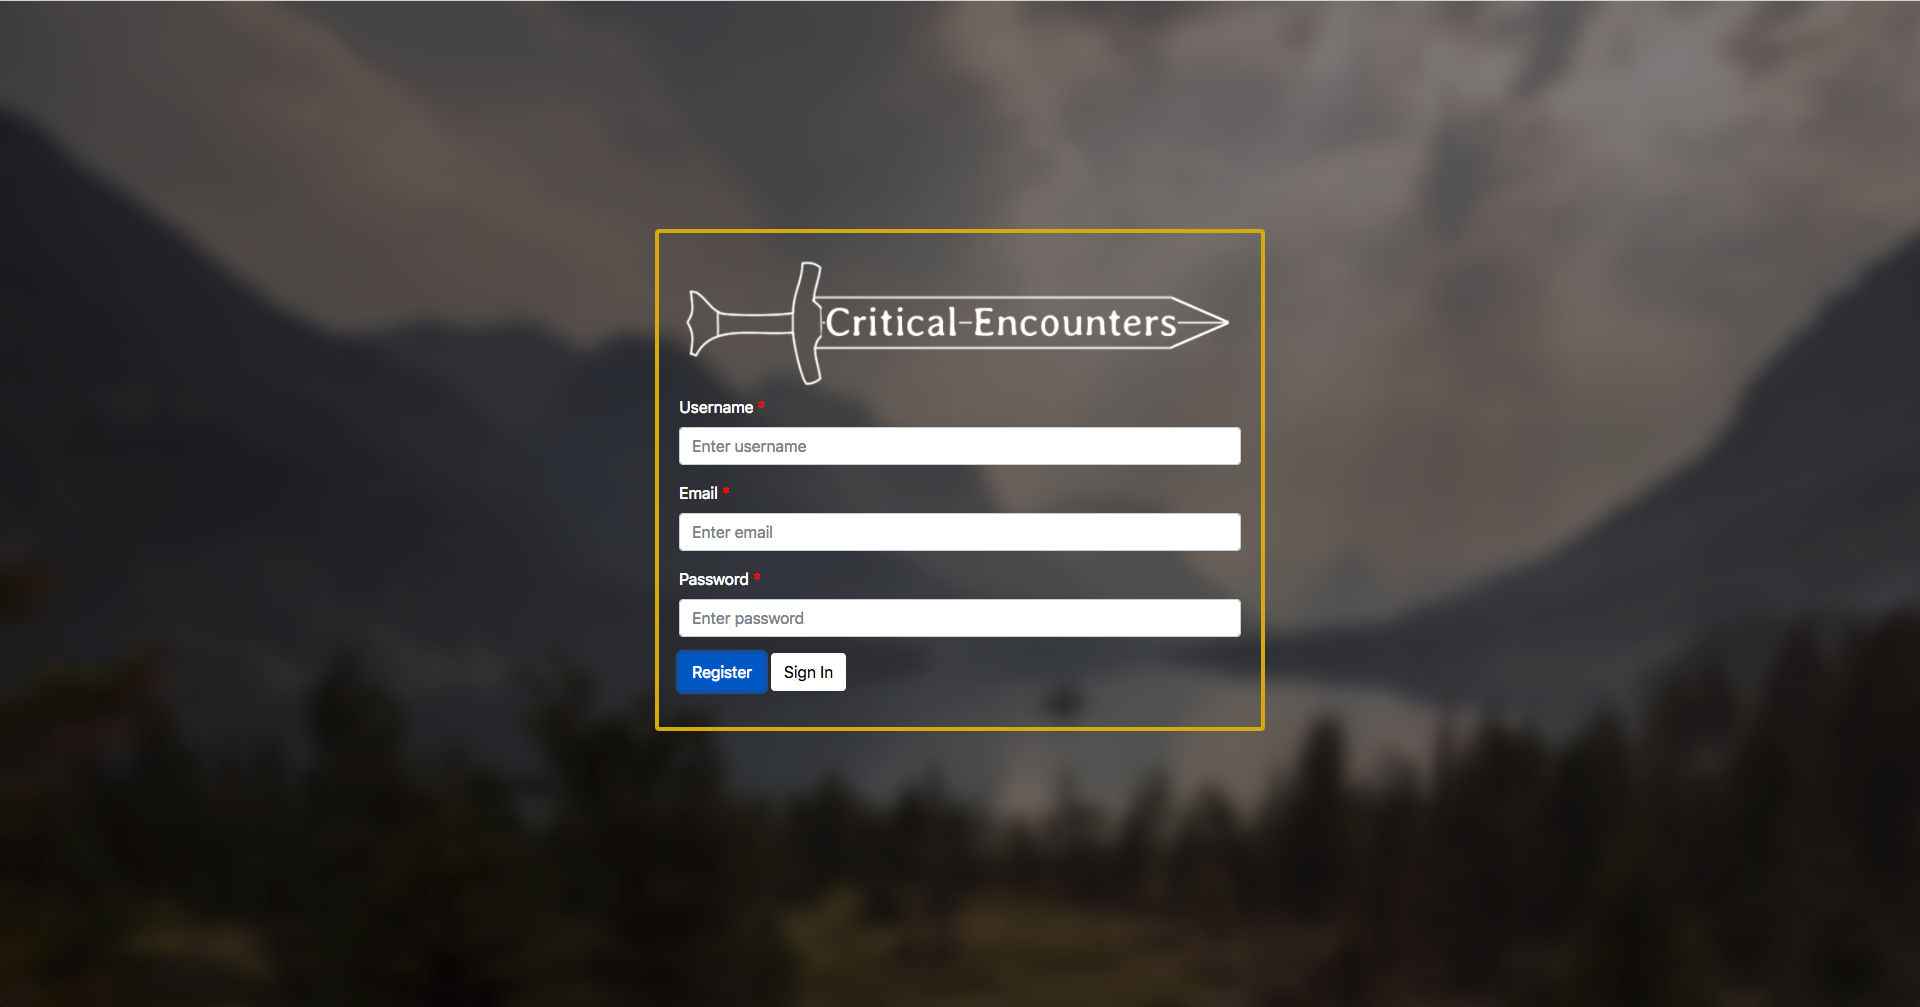
\includegraphics[scale=.20]{register}
		\caption{Registration Page}
		\label{fig: Registration Page}
	\end{figure}
		\newpage
	\section{Login Page}
	\begin{figure}[H]
		\centering
		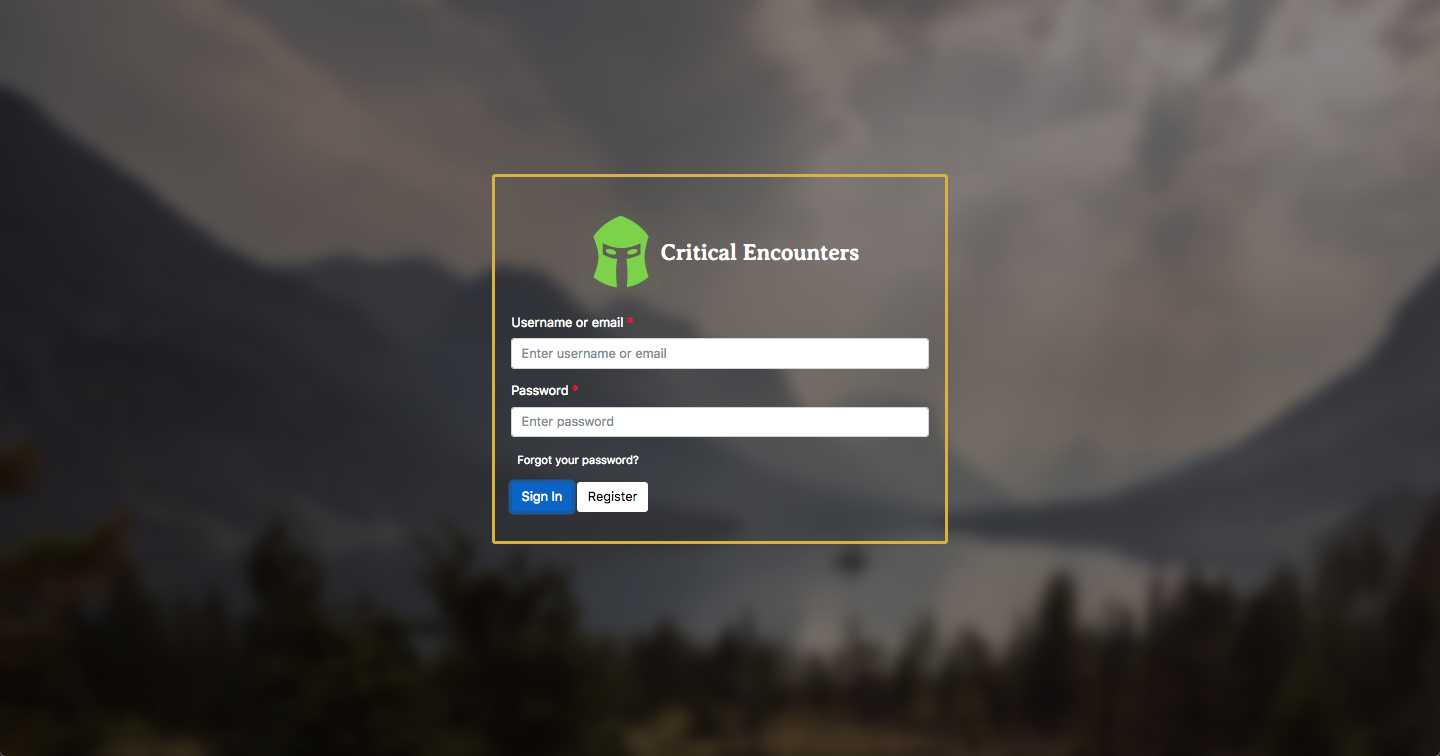
\includegraphics[scale=.20]{login}
		\caption{Login Page}
		\label{fig: Login Page}
	\end{figure}
	\newpage
	\section{Dashboard}
	\begin{figure}[H]
		\centering
		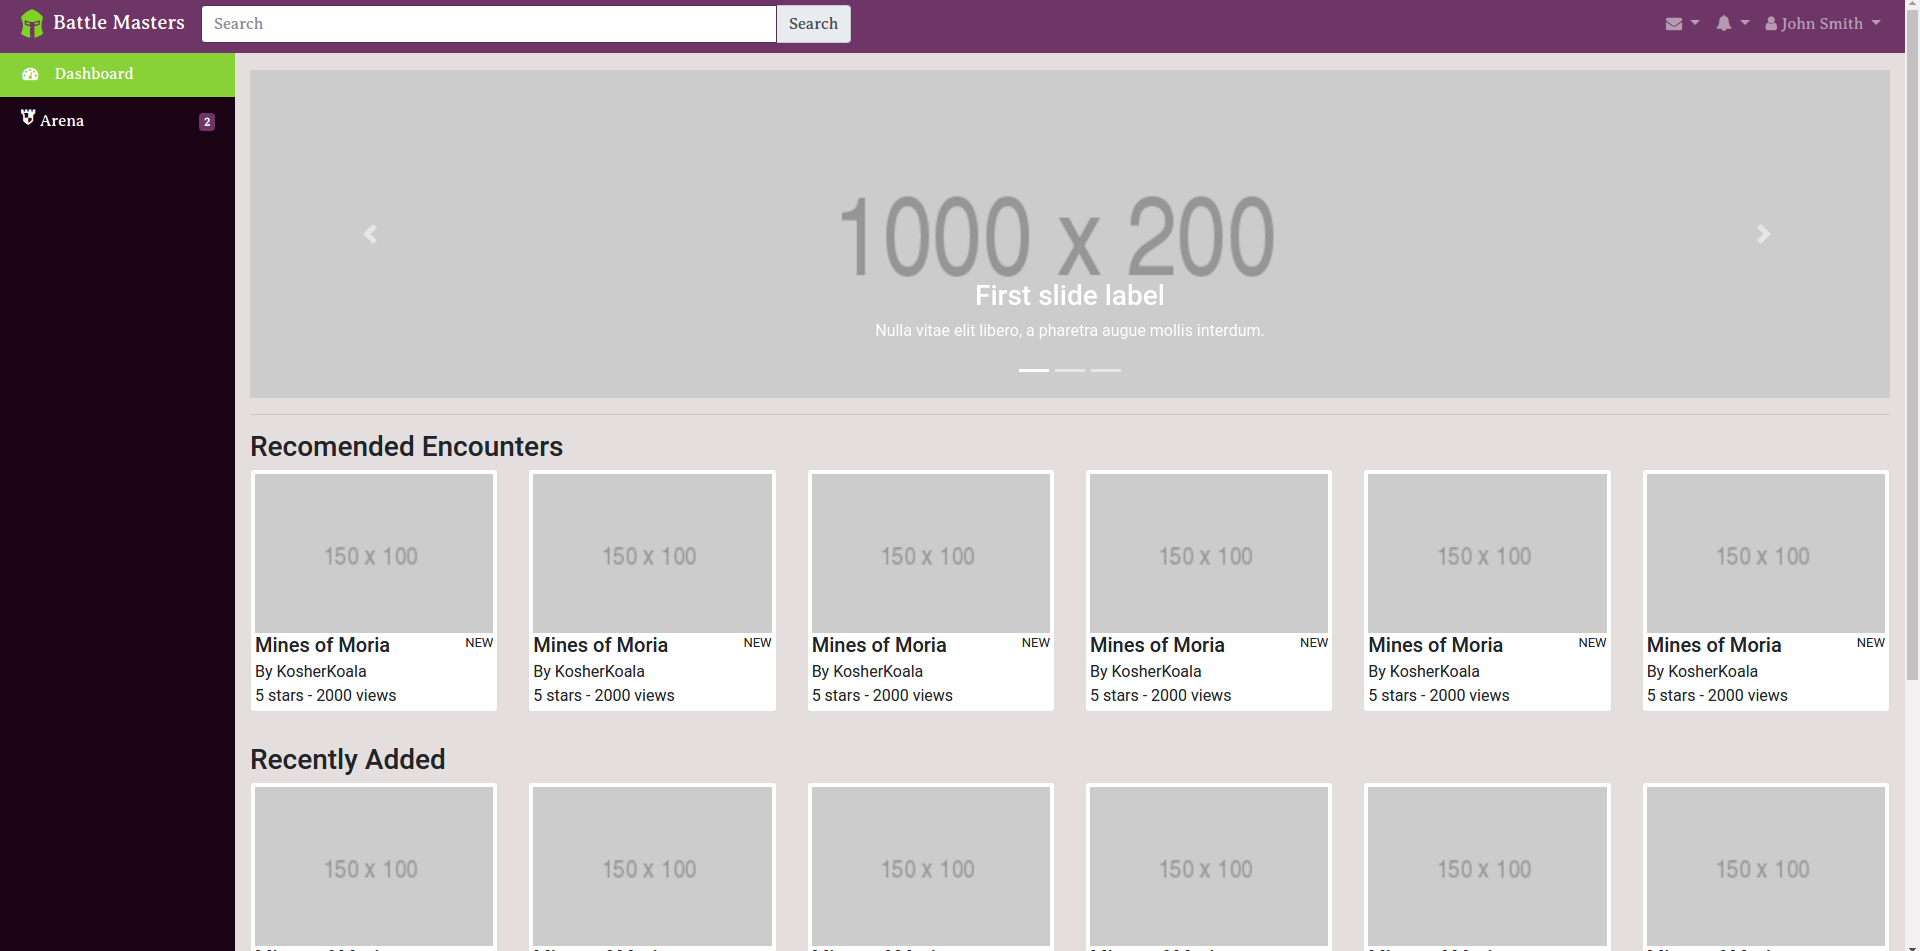
\includegraphics[scale=.20]{home}
		\caption{Dashboard}
		\label{fig: Dashboard}
	\end{figure}
	\newpage
	\section{Encounter Browser}
	\begin{figure}[H]
		\centering
		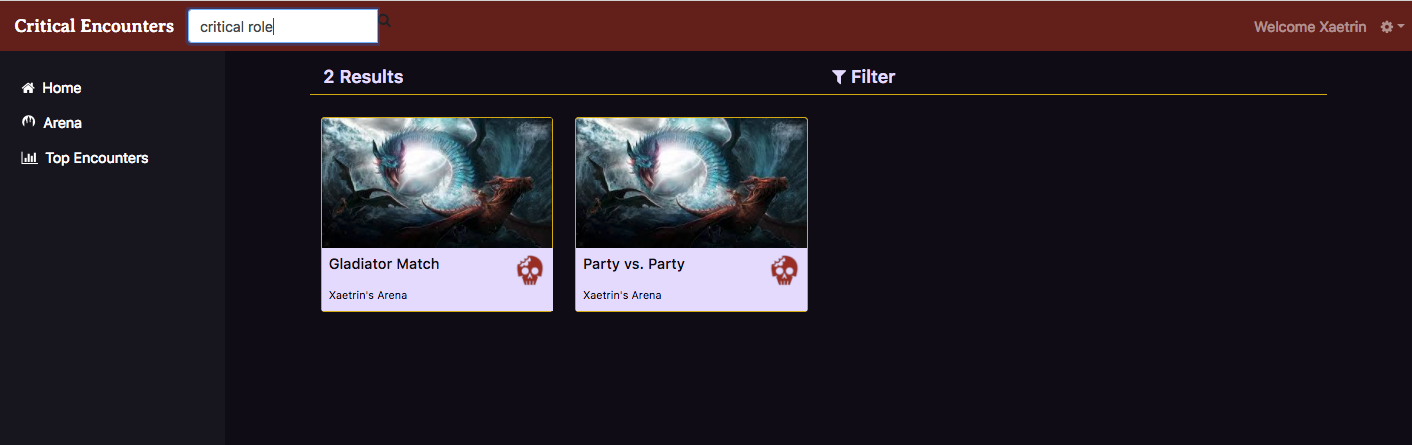
\includegraphics[scale=.19]{search}
		\caption{Encounter Browser}
		\label{fig: Encounter Browser}
	\end{figure}

	\begin{figure}[H]
		\centering
		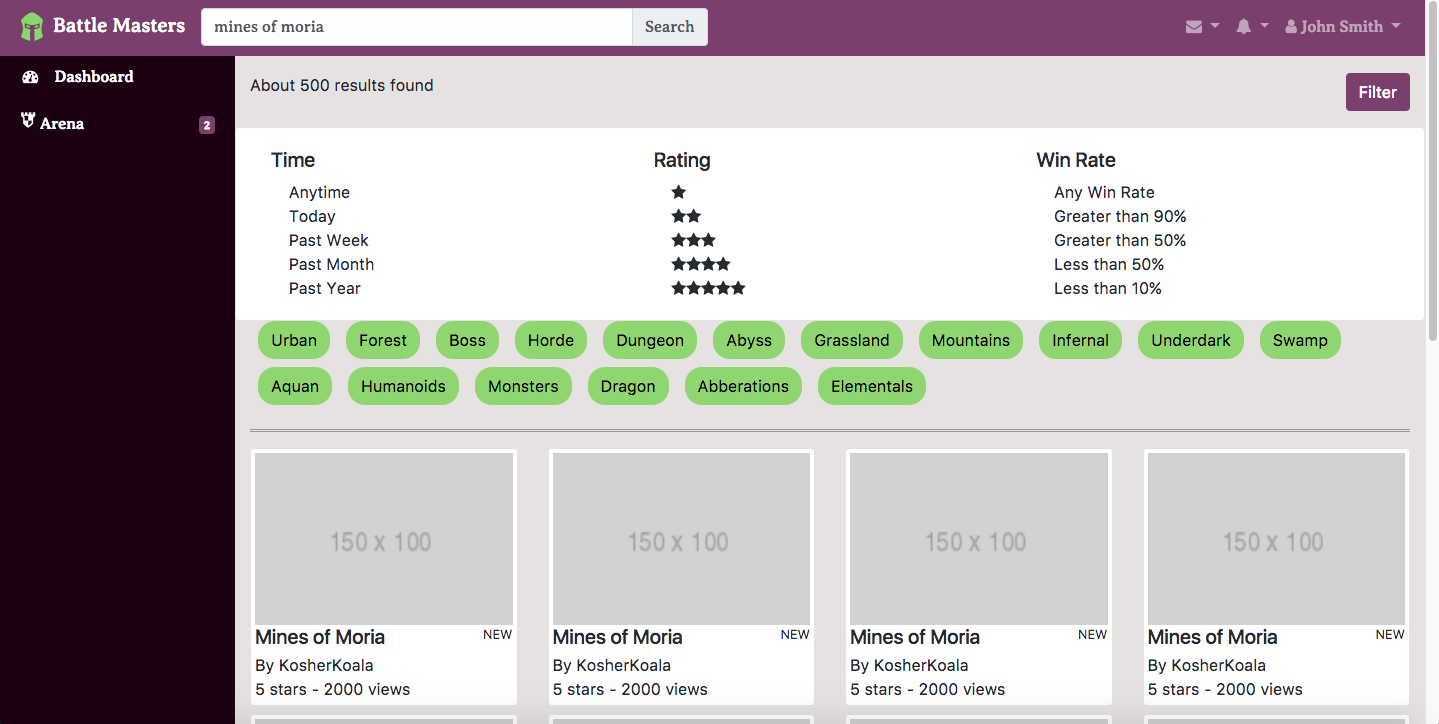
\includegraphics[scale=.25]{search_filtered}
		\caption{Encounter Browser with Filter Options}
		\label{fig: Encounter Browser with Filter Options}	
	\end{figure}
	\newpage
	\section{Arena}
	\begin{figure}[H]
		\centering
		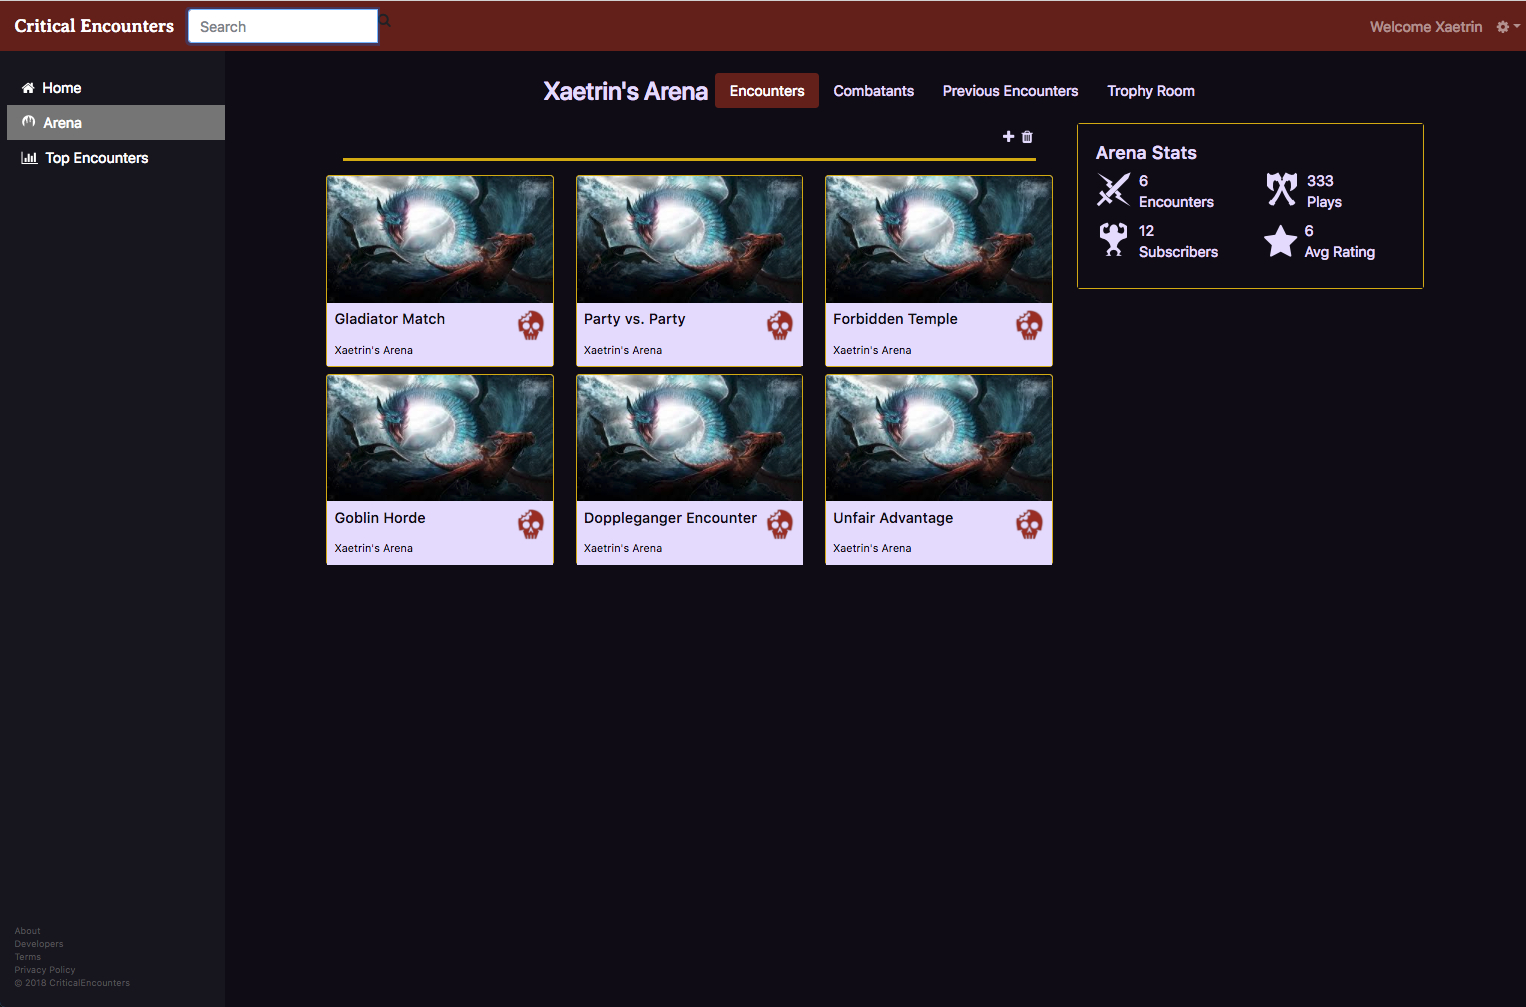
\includegraphics[scale=.20]{arena}
		\caption{Arena}
		\label{fig: Arena}
	\end{figure}
	
	\newpage
	\section{Encounter Page}
	\begin{figure}[H]
		\centering
		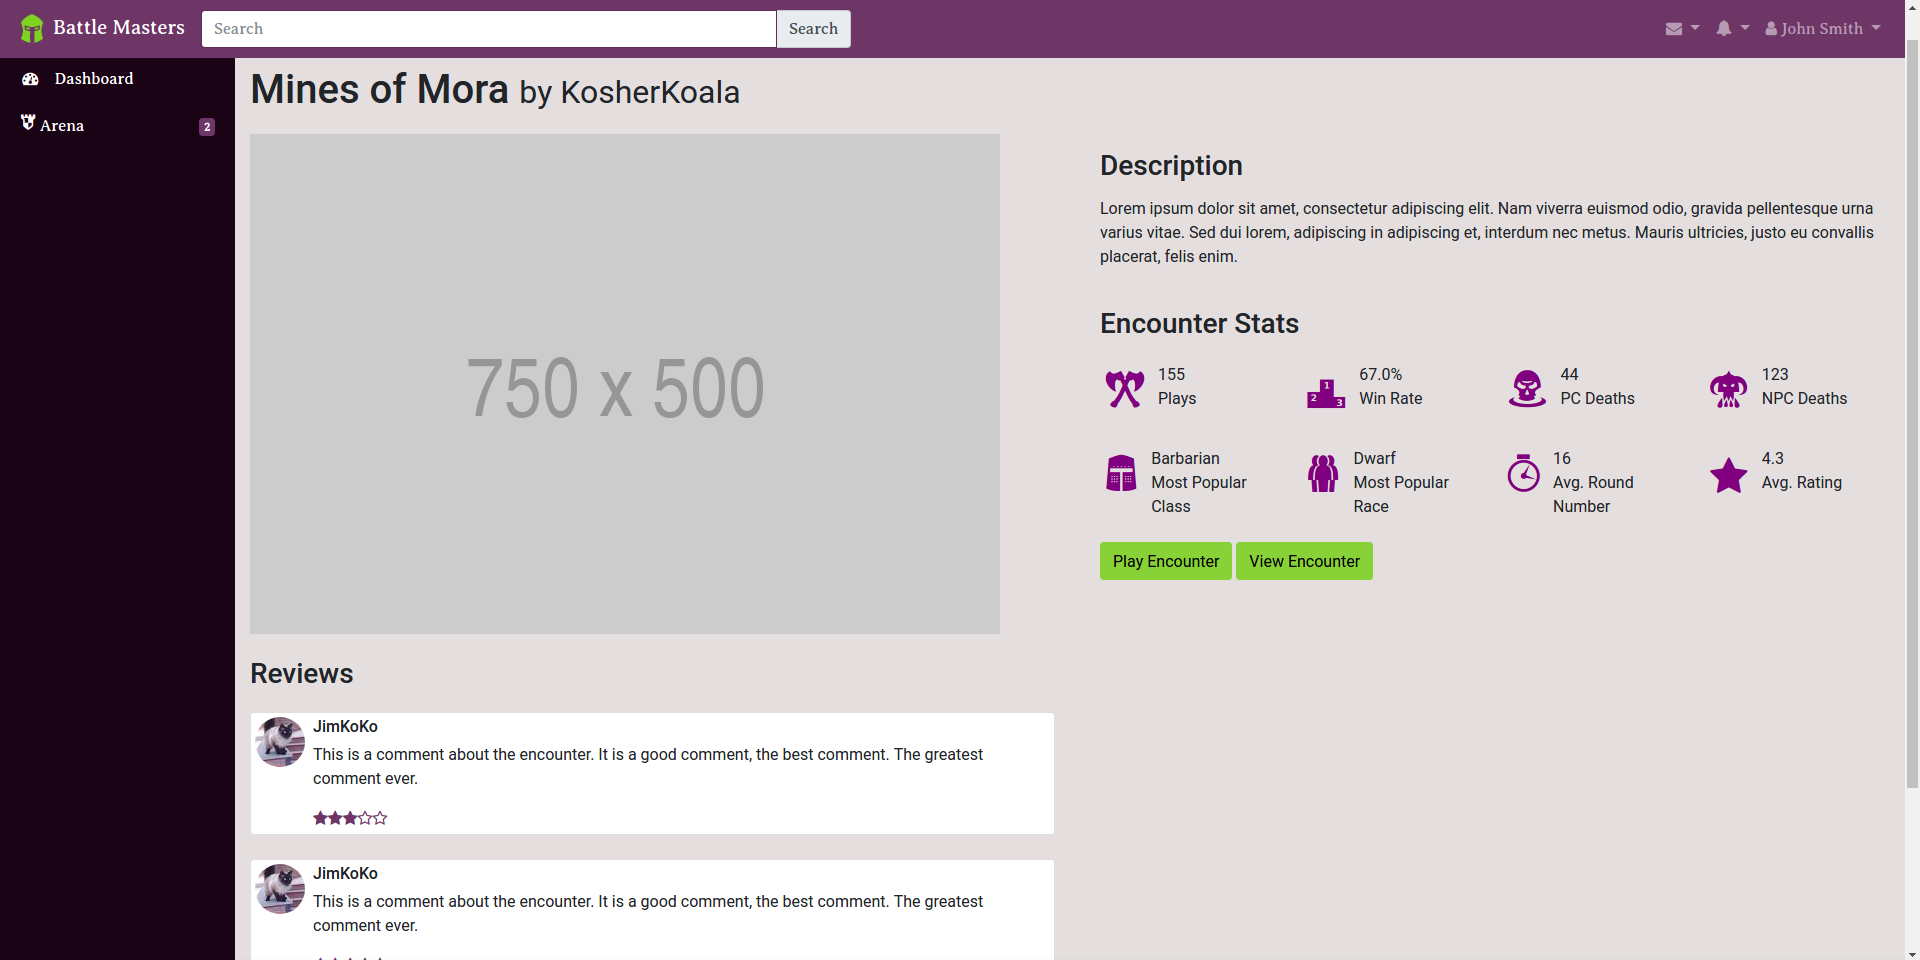
\includegraphics[scale=.20]{encounter}
		\caption{Encounter Page}
		\label{fig: Encounter Page}
	\end{figure}

	\newpage
	\section{Color Scheme}
	\begin{figure}[H]
		\centering
		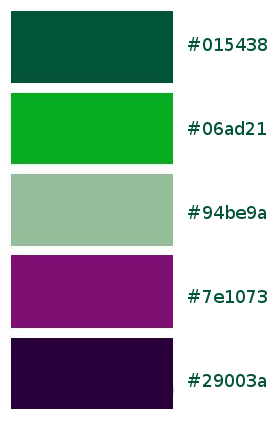
\includegraphics[scale=.5]{colors}
		\caption{Color Scheme}
		\label{fig: Color Scheme}
	\end{figure}
	\lipsum[4]
	\newpage
	\section{Icons}
	Most of the icons we utilize will be provided by the free icon APIs font-awesome and rpg-awesome. Additional icons will be acquired through Game-Icons.net.

	\subsection {Logo}
	\begin{wrapfigure}{l}{0\textwidth}
		
\includegraphics[scale=.5]{logo-large}
		\caption{Critical Encounters' Logo}
		\label{fig: Critical Encounters' Logo}
	\end{wrapfigure}
	We wanted the logo design to accompany the overall UI of the website with a simplistic design, while also representing the RPG aspect of Critical Encounters. We decided on a helmet because it gave a little more of a human feel, we thought swords or other weapons would be too inanimate. We chose the green color so the logo will "pop" with most backgrounds.This logo can also be easily scaled to fit most container sizes.
\newpage

	
\newpage
\chapter*{Application Design}
\stepcounter{chapter}
\addcontentsline{toc}{chapter}{Application Design}
	\section {High Level Design}
		\begin{figure}[h]
			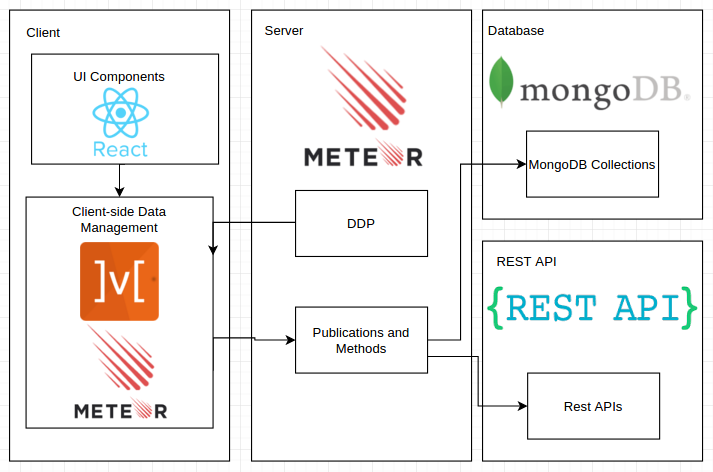
\includegraphics[scale=.5]{designsd.png}
			\caption{High Level Design Diagram}
			\label{fig: High Level Design}
		\end{figure}
		
		\paragraph{}We will be implementing a Client-Server Design structure that is commonly used with web apps such as Critical Encounters. There are three areas of production in this high-level design: Server, Database/Rest API and Client-Side. The UI components will be developed in REACT and will control the the MVC system. Data management on the client-side will be managed by MobX and Meteor, the latter of which will server as the point of contact with the server-side of the app. The server will also be developed in Meteor, and will be responsible for contacting the database, developed in MongoDB and performing REST API commands when necessary. 
		
		\paragraph {} The relationship between client and server will be a sudo model-view-controller architecture. Where REACT will act as the as application's view and Meteor/MobX will act as both the controller and the model. Meteor with MobX will automatically manage the data flow, client state, and client rendering.
	
	\section { Design Patterns }
		
		\begin{figure}[h]
			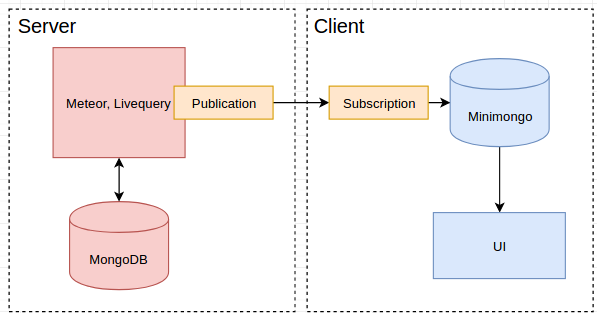
\includegraphics[scale=.7]{orm.png}
			\caption{Design Pattern Figure}
			\label{fig: Dasign Pattern }
		\end{figure}
		
		\paragraph{} Meteor uses implements a ORM/MERN, Object-relational mapping / MongoDB - Expess - React, stack design pattern. It focuses on model driven development, in which the models are shared between the server and the client. This is seen most clearly seen in the MiniMongo database cache that is accessible by the font-end front end and can asynchronously update the MongoDb REST API is implemented automatically which translates to automatic database updates.
		


\newpage
\section {Server Design}
	\subsection{Meteor}
		\begin{wrapfigure}{l}{0\textwidth}
			
\includegraphics[scale=.2]{meteorJS}
			\caption{Meteor.js}
			\label{fig: Meteor.js}
		\end{wrapfigure}
		Meteor is a full-stack JavaScript platform for developing modern web and mobile applications. Meteor includes a key set of technologies for building connected-client reactive applications, a build tool, and a curated set of packages from the Node.js and general JavaScript community.
		
		
		
		On the client, there is no direct connection to the MongoDB database, and in fact a synchronous API to it is not possible (nor probably what you want). Instead, on the client, a collection is a client side cache of the database. This is achieved thanks to the Minimongo library—an in-memory, all JS, implementation of the MongoDB API. What this means is that on the client, when you write:
		
		
		
		\begin{tabular}{ |p{3cm}||p{3cm}|p{3cm}|p{3cm}|  }
			\hline
			\multicolumn{4}{|c|}{Meteor Database} \\
			\hline
			Country Name     or Area Name& ISO ALPHA 2 Code &ISO ALPHA 3 Code&ISO numeric Code\\
			\hline
			Afghanistan   & AF    &AFG&   004\\
			Aland Islands&   AX  & ALA   &248\\
			Albania &AL & ALB&  008\\
			Algeria    &DZ & DZA&  012\\
			American Samoa&   AS  & ASM&016\\
			Andorra& AD  & AND   &020\\
			Angola& AO  & AGO&024\\
			\hline
		\end{tabular}
		
	\subsection{Server Sequence Diagrams}

\newpage
\section{Database Design}
	\subsection{Schema}
		Below are schema that will be used to structure the MongoDB collections. The schema themselves will be implemented in Meteor using their MongoDB schema syntax and design. Below is an example of the schema representation of a Critical Encounter user collection:
		
		\begin{lstlisting}
			Users.schema = new SimpleSchema({
				username: {type: String, required: true},
				password: {type: String, required: true},
				arena: {type: String, regEx: SimpleSchema.RegEx.Id},
				subscriptions: [{type: String, regEx: SimpleSchema.RegEx.Id}]
			});
		\end{lstlisting}
		
		The general structure is a field name and a matching feild type (String, Boolean, Object ) with optional requirements or parameters (regEx: SimpleSchema.RegEx.Id).
		
		Note: The { "Collection Name" } notation represents an Object.id that correlates to a MongoDB object of that collection type
		\subsubsection{User Schema}
			\begin{figure}[h]
				\centering
				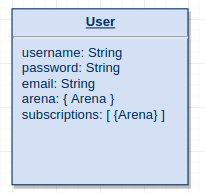
\includegraphics[scale=.75]{schema-user}
				\caption{User Schema}
				\label{fig: User Schema }
			\end{figure}
			
		\paragraph{}This schema will hold basic user information: identification information (username, password), a reference to their Area (Arena), and a list of the Arenas they are subscribed to (subscriptions). This is the entrance point for all data accessible on the website. All other collections on the database are associated with at least one user object and has only one user owner/creator. All login and authentication information and routing will referenc the user collection to confirm identification. The password string will be saved as a string that has been encrypted to protect user information.
		\subsubsection{Arena Schema}
		
			\begin{figure}[h]
				\centering
				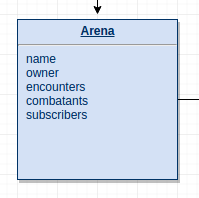
\includegraphics[scale=.75]{schema-arena}
				\caption{Arena Schema}
				\label{fig: Arena Schema }
			\end{figure}
		
			\paragraph{}This schema will hold basic Arena information: an Arena name (name), a reference to Arena's creator: (owner), a list of encounters that are contained in the arena (encounters), and a list of references to users that are subscribed to the (subscribers). The Arena acts as a hub, organizer and access or for every user and their encounters. Arena statistics are not directly maintained in the Area object itself but are compiled from the list of encounters that is contained in the encounters field. This allows the statistics as up to date as possible without constantly updating both area statistic and the encounter statistics when an encounter goes through a stat change.
		\subsection{Encounter Schema}
			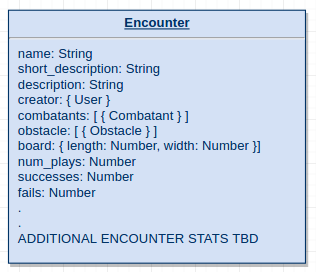
\includegraphics[scale=.75]{schema-encounter}
		\subsection{Combatant Schema}
		\subsection{Obstacle Schema}
			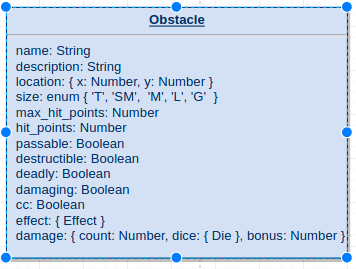
\includegraphics[scale=.75]{schema-obstacle}
		\subsection {Spell Schema}
			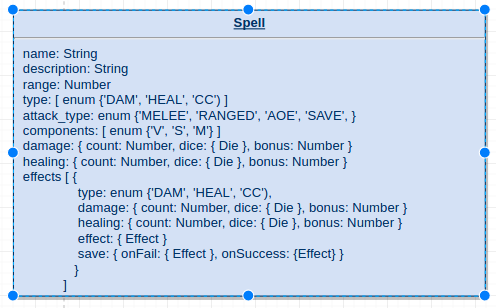
\includegraphics[scale=.75]{schema-spell}

\newpage
\section{Client Side Design}
	\subsection{URL and Routing}
		\paragraph {} There are two options to font-end routing for using our stack: React-Router and Meteor's FlowRouter. Both implementations have their pros and cons but after some research and deliberation we have decided to use Meteor's FlowRouter. The notation and syntax for FlowRouter is much more clear and easier to learn. There haws also been a history of React-Router not playing too well with Meteor applications. 
		
		FlowRouter is relatively straight fore-ward and is composed of two main components, the URL and the action. In short when the URL is accessed by the browser the action is triggered. In our case the action method will most likely be a ReactLayout render call to render react components associated with that route to the view. 
		
		Below is a routing example for the dashboard page of Critical Encounters:
		
		\begin{lstlisting}
			FlowRouter.route( '/dashboard', {
				name: 'dashboard',
				action() {
							ReactLayout.render( App, { yield: <DashBoard /> } );
				}
			});
		\end{lstlisting}
		
		\subsubsection { URL Routes}
		
			\begin{table}[H]
				\begin{center}
					\begin{tabular}{ |p{5cm}|p{7cm}|| } 
						\hline
						URL Route: & Purpose: \\
						\hline
						/dashboard & Routes users to dashboard page \\
						/account & Routes current user account information\\
						/encounter-finder/:query & Route to search result page accessible at anytime through the fixed header search bar  \\
						/arenas/:arenaName & Route to area with specified arena name  \\
						/encounters/:id & Route to encounter with specified id \\
						/battlefield/creator/:id & Enter Battlefield in creator mode with given encounter id \\
						/battlefield/player/:id & Enter Battlefield in player mode with given encounter id \\
						/battlefield/master/:id & Enter Battlefield in master mode with given encounter id \\	
						\hline
					\end{tabular}
				\end{center}
			\caption{URL Routes} \label{table: URL Routes}
		\end{table}
		
		
	\subsection{Types of Views and Controllers}
	\subsection{Battlefield Modes}
		\subsubsection{Game Mode}
			This is the main mode available in DMBD. In this mode users will be able to play, simulate, and view and gather data about their and other user's encounters.
			\subsubsection{Roles}
				\paragraph{Player}
					Player is in control of a single player character and can either control his character directly in combat or apply an AI to his player character. every round the player will perform his/her character's actions on its turn. Once complete the AI will simulate all other combatant's turns and refresh the battlefield. Once the encounter is complete the player will be able to view his character's stats and results from the encounter.
				\paragraph {Game Master} Controls multiple combatants against a one or more player characters. The game master on each turn can choose to either simulate the combatant's turn or perform the actions on the combatant's turn manually using the AI. After the encounter has completed there the game master will be able to review the encounter stats and results.
				
		\subsection{Creation Mode}
			\subsubsection{Roles}
				\paragraph There is only one role available for the Creation Mode: Creator. In this mode the user will be able to design their own encounters using the Encounter Creator Tools. Users will be able to add obstacles and combatants, as well as customize the combatants stats and AI presets. Once the user has completed creating the encounter the user may either publish the encounter, and perform Encounter Validation process or keep the encounter private for personal or invite use.
	\subsection{Map / Environments}
	
	\subsection{Turn Structure / Order}
	Combat using the d20 System is composed of rounds in which each combatant in the encounter has one turn.  A round lasts 6 seconds in game time, during which all combatants act on their respective turns. Where a combatant's turn resides chronologically in a round is determined by the combatant's initiative roll (a combination of a dice roll and applicative bonuses). A turn it self is composed of 6 parts: Action(s), Bonus Action, Movement, Free Action, and Bonus Action, Reaction.
	\begin{itemize}
		\item Action
			\begin{itemize}
				\item The main action of a turn, every combatant has one or more per turn
				\item Ex. Attack, Cast a Spell, Dash, Disengage, Hide
			\end{itemize}
		\item Bonus Action
			\begin{itemize}
				\item An action gained by a feature, spell, or other abilities
				\item Ex: The Cunning Action feature allows a rogue to take a Bonus Action to hide, dash, or disengage
				\item Max one Bonus Action per turn
			\end{itemize}
		\item Movement
			\begin{itemize}
				\item Combatant can move the number of spaces equal to its speed (with applicaple bonuses) divided by five
				\item Some combatants also have swim and flight speeds that they can use as their movement action
				\item Multiple environmental restraints on this: Difficult terrain, attacks of opportunity
			\end{itemize}
		\item Free Action
			\begin{itemize}
				\item Interact with one object or environment 
				\item Ex: Open a door, you could draw your weapon
				\item interaction with more than one action requires the use of an action
			\end{itemize}
		\item Reaction
			\begin{itemize}
				\item Combatant has one of reaction in every round of combat
				\item Can happen anytime during the round, doesn't have to be combatant's turn
				\item Ex. Cast reaction spell, attack of opportunity
			\end{itemize}
	\end{itemize}

\newpage
\chapter*{Research}
\stepcounter{chapter}
\addcontentsline{toc}{chapter}{Research}
			\subsubsection{Bootstrap 4}
			\begin{wrapfigure}{r}{0\textwidth}
				
\includegraphics[scale=0.1]{bootstrap4}
				\caption{Bootstrap 4}
				\label{Bootstrap 4}
			\end{wrapfigure}
			Bootstrap is a HTML, CSS, and JS framework used for building responsive, mobile compatible web sites and applications. Bootstrap was an obvious choice for out front end development. It has extensive documentation and resources available. Also with its new v4 update Bootstrap is more useful then ever. Our front end team already has extensive experience with Bootstrap so it should be easy to get the front end up and running. The tricky aspect of this will be the transition from experience with Angular to now using React.js. We decided to make this transition because of the popularity and momentum React is having in the web development community, to both widen our gaze and take advantage of many features that using Bootstrap with React has to offer.


	
\end{document}